\chapter{Deep Learning For Simulation}
    Deep Learning, as a branch of Machine Learning, employs algorithms to process data and imitate the thinking process\cite{schmidhuber2015deep}, or to develop abstractions. Deep Learning (DL) uses layers of algorithms to process data, understand human speech, and visually recognize objects. Information is passed through each layer, with the output of the previous layer providing input for the next layer. The first layer in a network is called the input layer, while the last is called an output layer. All the layers between the two are referred to as hidden layers. Each layer is typically a simple, uniform algorithm containing one kind of activation function.  \\
    \begin{figure}[!ht]
        \centering
        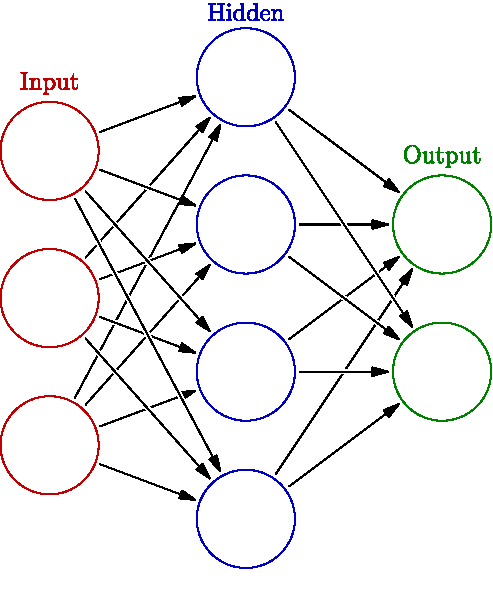
\includegraphics[scale = 0.5]{Figures/Colored_neural_network}
        \caption{visulization of one simple $3$-layers neural networks, including input layer, hidden layer and output layer, \textit{retrieved from Wikipedia}}
    \end{figure}

    With deep learning becoming more and more popular in many fields of researching, some classical methods can be replaced by deep learning. Many successful application of deep learning can be found in computer vision part, like image segmentation\cite{lecun2015deep},objection recognition\cite{he2016deep}. 

\section{Convolutional Neural Networks}
    \begin{figure}[!h]
        \centering
        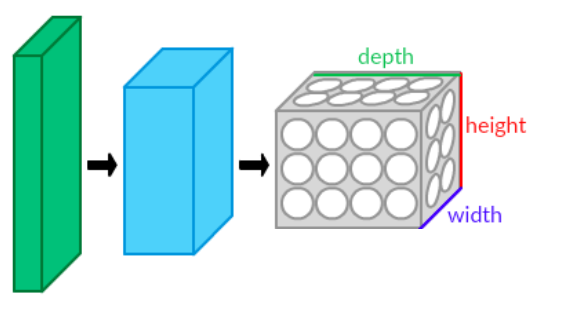
\includegraphics[scale = 0.5]{Figures/Conv_layers.png}
        \caption{Visualization of convolutions network, \textit{retrieved from Wikipedia}}
    \end{figure}

\section{CNN Constructure}
    \subsection{Convolutional layers}

    \subsection{Full-connected layers}

\section{Traing configuration}
    \subsection{Loss Function}

    \subsection{Optimizer(SGD)}

\section{Training Results}

\section{Simulation based on Trained model}